%!TeX root=MemoriaTFG.tex

\chapter{Contextualización}\label{contextualizacion}
% \todo{Esto es una prueba. Isaac}

Con el fin de tener una visión inicial antes de profundizar con el tema del trabajo, se explican brevemente los distintos conceptos necesarios para situarse en el contexto del proyecto, entre ellos: definición de la inteligencia artificial, tipos de inteligencia artificial, enfoques adaptados en su desarrollo e introducción a los conceptos de las redes neuronales.

\section{El mundo de la inteligencia artificial}

El concepto de \textbf{\textit{ente inteligente}} es un concepto que se lleva definiendo y redefiniendo desde hace siglos. Para los filósofos, serviría para definir la naturaleza del ser humano. Para los científicos, sería un medio por el cual se podrían llevar a cabo demostraciones lógicas impenetrables y cálculos extremadamente complejos para la resolución humana. Para los escritores, un ser fantástico y poderoso capaz de realizar cosas inimaginables, a menudo despertando el miedo en los lectores. \\

Sin embargo, en su esencia, es una \textit{expansión de las capacidades humanas}, una mejora, un mecanismo de resolución de tareas y problemas que facilitaría la vida en todos sus aspectos ~\cite{buchanan2005very}.

\subsection{¿Qué es la inteligencia artificial?}

La inteligencia artificial se define como la \textbf{capacidad de una máquina de simular el comportamiento y el razonamiento humano}, de tal manera que frente a cualquier situación razone y/o actúe de la misma manera que una persona haría. \\

La inteligencia humana está compuesta de tres tipos de ingeligencia distintas, algo de lo que Santiago Sánchez-Migallón, profesor de filosofía,, explicaba en un repaso de $"$\textit{qué hace al ser humano inteligente}$"$ \cite{pastor2008inteligencia}: 

\begin{enumerate}
    \item \textbf{Inteligencia componencial}, nuestra capacidad de análisis: dirección consciente de nuestros procesos mentales para analizar y evaluar ideas, resolver problemas y tomar decisiones.
    \item \textbf{Inteligencia experiencial}, nuestra creatividad: capacidad de afrontar tareas novedosas, formular nuevas ideas y combinar experiencias.
    \item \textbf{Inteligencia práctica o contextual}, capacidad de adaptación al medio: adaptación, selección o modificación del ambiente individual. Realmente, esta es la inteligencia más importante (si bien depende de las otras dos), ya que tu éxito o fracaso  dependerá de ella. 
\end{enumerate}


Para que una máquina sea inteligente, esta debe: 

\begin{enumerate}
    \item Tener la habilidad de \textbf{\textit{razonar}}. El razonamiento puede ser \textbf{inductivo} o \textbf{deductivo}:
        \begin{enumerate}
            \item En el razonamiento deductivo la veracidad de las premisas \textit{garantiza} la veracidad de la conclusión.
            \item En el razonamiento inductivo las premisas verdaderas \textit{apoyan} la veracidad de la conclusión pero sin asegurarla.
        \end{enumerate}
    \item Poder \textbf{\textit{analizar}} el entorno, \textbf{\textit{entender las percepciones}} recibidas y, a partir de éstas, \textbf{\textit{determinar cómo debe actuar o comportarse a continuación}}.
    \item \textbf{\textit{Aprender de experiencias}} anteriores, de tal manera que tenga memoria de todas las interacciones que ha llevado a cabo.
    \item A partir de la experiencia, ser capaz de \textbf{\textit{generalizar conceptos}}; es decir, ser capaz de realizar conexiones de causa y consecuencia, reglas internas que expliquen el por qué de las percepciones que recibe y ser capaz de reconocer las percepciones que son iguales.
\end{enumerate}

\subsection{Tipos de inteligencia artificial}

Según Stuart Russell y Peter Norvig, autores del libro \textit{Inteligencia Artificial: Un enfoque moderno} \cite{russell2002artificial}, hay 4 tipos distintos de inteligencia artificial \cite{russell2002artificial, iaWikipedia}:
\begin{enumerate}
    \item Sistemas que \textbf{\textit{piensan} como humanos} - estos sistemas tratan de reproducir el pensamiento humano. A esta categoría pertenecen las redes neuronales artificiales. Entre las actividades que se pueden llevar a cabo con estos sistemas son la toma de decisiones, la resolución de problemas y el aprendizaje.
    \item Sistemas que \textbf{\textit{actúan} como humanos} - estos sistemas tratan de imitar el comportamiento humano. Un ejemplo de sistemas de este tipo es la robótica.
    \item Sistemas que \textbf{\textit{piensan} racionalmente} - estos sistemas tratan de imitar o emular el pensamiento lógico racional del ser humano. Un ejemplo de estos sistemas son los sistemas expertos (como \textit{MYCIN} \cite{shortliffe2012computer}).
    \item Sistemas que \textbf{\textit{actúan} racionalmente} - tratan de emular de forma racional el comportamiento humano. A esta última categoría pertenecen los agentes inteligentes, y es el tipo de inteligencia artificial que se ha estado desarrollando para el TFG.
\end{enumerate}

\subsection{Enfoques de la inteligencia artificial}

Existen dos tipos de enfoques que se siguen cuando se desea implementar un sistema inteligente \cite{copeland2020ai}:
\begin{enumerate}
    \item Simbólico, o \textit{\textbf{descendente}}: se quiere replicar la inteligencia mediante premisas definidas. Según la hipótesis formulada por Newell y Simon (\textit{physical symbol system hypothesis}) \cite{nilsson2007physical, newell2007computer}, \textit{$"$el procesamiento de estructuras de símbolos es suficiente, teóricamente, para producir inteligencia artificial en un ordenador digital y que, además, la inteligencia humana es el resultado del mismo tipo de manipulación simbólica.$"$}
    \item Conexionista, o \textit{\textbf{ascendente}}: se pretende emular las capacidades y el comportamiento del cerebro humano mediante procesos que emergen de redes formadas por unidades sencillas interconectadas (como las neuronas). Las redes neuronales artificiales han sido creadas para que repliquen las conexiones del cerebro humano, de ahí el término \textit{conexionista}. En la siguiente sección se explicará más detenidamente este enfoque. 
\end{enumerate}

\section{Machine Learning. El aprendizaje en inteligencia artificial}


\textbf{\textit{Aprendizaje automático}}, o (\textit{Machine Learning}), hace referencia a la capacidad de una máquina, software u aplicación de aprender mediante la aplicación de algoritmos específicos a cierta entrada de datos de su sistema de manera independiente \cite{apd2019ml}. \\

El \textbf{Aprendizaje Automático} consiste en una disciplina de las ciencias informáticas, relacionada con el desarrollo de la Inteligencia Artificial, y que sirve, como ya se ha dicho, para crear sistemas que pueden aprender por sí solos. \\

Es una tecnología que permite hacer automáticas una serie de operaciones con el fin de reducir la necesidad de que intervengan los seres humanos. Como estas acciones se realizan de manera autónoma por el sistema, se dice que el aprendizaje es \textit{automático}.\\

El aprendizaje consiste en la capacidad del sistema de identificar una gran serie de patrones complejos determinados por una extensa cantidad de parámetros. Para que aprenda, el algoritmo interno del sistema se modifica con la constante entrada de datos en la interfaz, y puede, de ese modo, predecir escenarios futuros o tomar acciones de manera automática según ciertas condiciones.

\subsubsection{Funcionamiento del aprendizaje automático}
En los inicios de la informática, el único modo de conseguir que un sistema hiciera algo era escribiendo un algoritmo que definiera el contexto y detalles de cada acción, por lo que el proceso estaba completamente supervisado y controlado por un ser humano. \\

En cambio, los algoritmos que se usan en el desarrollo del \textit{Machine Learning} realizan buena parte de estas acciones por su cuenta. Obtienen sus propios cálculos según los datos que se recopilan en el sistema, y cuantos más datos obtienen, mejores y más precisas serán las acciones resultantes. \\

El éxito de un buen sistema de aprendizaje automático se encuentra en la construcción y adaptación de los árboles de decisiones en base a los datos previamente conocidos por el sistema. Sin embargo, también influye la \textbf{aplicación de fórmulas heurísticas} en los nodos que forman el árbol mediante las que elabora un sistema de inferencias. \\

El sistema de Machine Learning \textbf{necesita contar con un volumen de datos de relevancia para poder suministrar respuestas realmente válidas}. Es decir, cuantos más datos tiene para entrenar y con los que aprender, mejores predicciones, clasificaciones, análisis, etc. será capaz de realizar. Al igual que en la estadística, cuantos más muestras se tenga de la población más se podrá generalizar y crear un sistema que sea capaz de reconocer el mayor número de casos posibles \cite{estadisticaDescriptiva, estadisticaGeneralizar, fernandez2002estadistica}. 

\subsection{Tipos de aprendizaje}

Un sistema de aprendizaje automático utiliza sus experiencias y las evidencias de su entorno como datos para identificar y analizar por sí mismo patrones, comportamientos, relaciones del entorno, etc. De esta manera, adquiere una capacidad de elaborar predicciones de escenarios o iniciar operaciones que son la solución para una tarea específica. \\

A partir de un gran número de ejemplos de un mismo escenario se puede elaborar \textbf{un modelo que deduzca y generalice el comportamiento observado}. Una vez construido el modelo se podrán realizar predicciones para casos totalmente nuevos. \\

El entreno al fin y al cabo es la forma que tiene la red de \textbf{aprender}, de convertirse en \textit{inteligente}. El aprendizaje en inteligencia artificial es uno de los pilares más importantes, y existen tres categorías distintas: el \textbf{aprendizaje supervisado}, el \textbf{aprendizaje no supervisado}, y el \textbf{aprendizaje por refuerzo}. En la Fig. ~\ref{fig:ml_tipos_aprendizaje} se muestran todas las aplicaciones de cada uno de los aprendizajes. 
 
\begin{figure}[h]
    \centering
    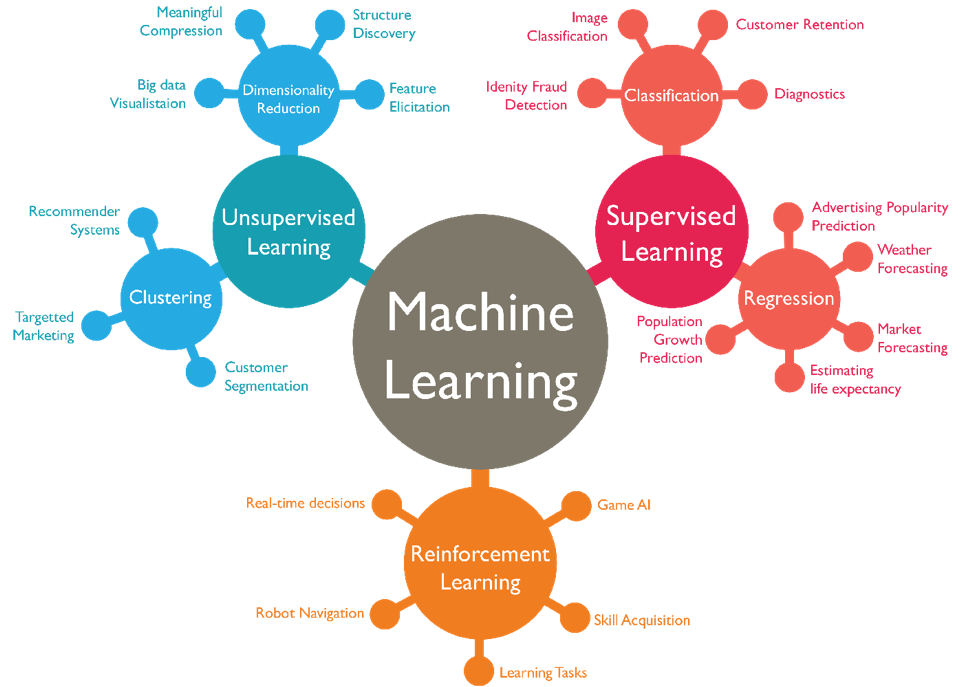
\includegraphics[scale=0.5]{cap2_contextualizacion/images/ml_learning.png}
    \caption{Tipos de aprendizaje en Machine Learning (Fuente: ~\cite{chugh2008mltypes}).}
    \label{fig:ml_tipos_aprendizaje}
\end{figure}


\subsubsection{Aprendizaje supervisado}

El \textit{aprendizaje supervisado} se basa en la existencia de \textbf{\textit{muestras etiquetadas}} con las que el modelo aprende a identificar los distintos ejemplos que se los proporciona por sus etiquetas: aprende a \textit{clasificarlos}. Para hacer un símil con la naturaleza humana, es como estar enseñándole un objeto a un niño  y diciéndole qué es para que lo pueda reconocer en un futuro. \\

Una vez que se le ha proporcionado la suficiente cantidad de dichos datos, podrán introducirse nuevos datos sin necesidad de etiquetas, en base a patrones distintos que ha venido registrando durante el entrenamiento. Este sistema se conoce como \textit{clasificación}. \\

Otro método de desarrollo del Aprendizaje Automático consiste en predecir un valor continuo, utilizando parámetros distintos que, combinados en la introducción de nuevos datos, permite predecir un resultado determinado. Este método se conoce como \textit{regresión}. \\

Lo que distingue al Aprendizaje Supervisado es que se utilizan distintos ejemplos a partir de los que generalizar para nuevos casos. 

\subsubsection{Aprendizaje no supervisado}

En cambio, en el \textit{aprendizaje no supervisado} se entrena con datos sin etiquetas - el modelo analiza los datos y se crea él sus propias etiquetas, sus propios grupos, según distintos estrategias de análisis (por distancia, generalmente). \\

Estos sistemas tienen como finalidad la comprensión y abstracción de patrones de información de manera directa, concepto que se conoce como \textbf{\textit{clustering}}.

Este tipo de aprendizaje es más complejo que el anterior, pero es capaz de encontrar relaciones y patrones en los datos que los humanos no serían capaces de reconocer. \\

Un ejemplo de aplicación de este aprendizaje es la clasificación de los compradores en base a sus intereses y a su historial de compras. Este análisis podría mostrar una relación entre la información demográfica de una persona y sus tendencias de compras. \\

\begin{figure}[h]
    \centering
    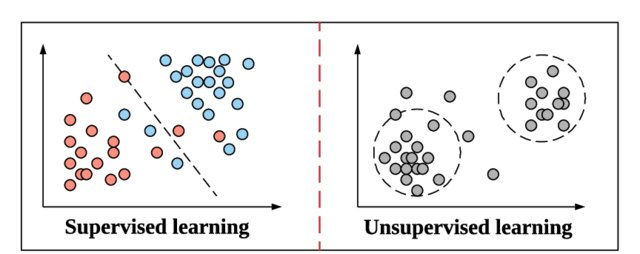
\includegraphics[scale=1]{cap2_contextualizacion/images/diff_sup_unsu.jpg}
    \caption{Aprendizaje supervisado vs. no supervisado.}
    \label{fig:diff_sup_unsu}
\end{figure}

\subsubsection{Aprendizaje por refuerzo}

En la técnica de \textit{aprendizaje por refuerzo} el aprendizaje se realiza por medio de la \textbf{\textbf{prueba y error}}, por lo que los sistemas aprenden completamente a partir de la experiencia - sin intervenciones humanas ni datos con etiquetas. Mediante el uso de funciones de premio que optimizan su comportamiento, el sistema se consigue ser \textbf{\textit{totalmente autónomo}}. \\

\begin{figure}[h]
    \centering
    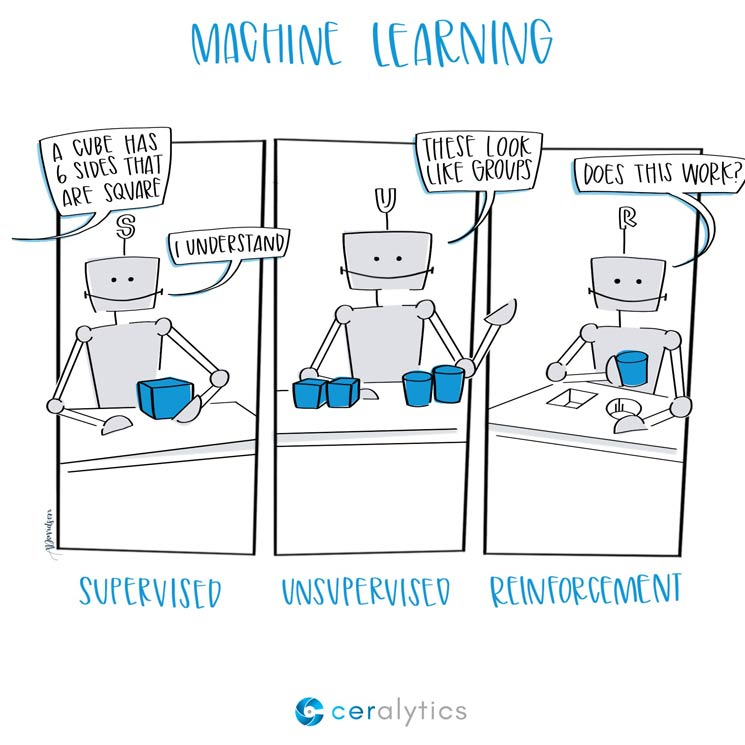
\includegraphics[width=0.45\textwidth]{cap2_contextualizacion/images/machine-learning_ceralytics.jpg}
    \caption{Cómo se diferencian los distintos tipos de aprendizaje en Machine Learning (Fuente: ~\cite{ceralyticsMLtypes}).}
    \label{fig:ml_ceralytics}
\end{figure}

A modo de resumen, en la Fig. ~\ref{fig:ml_ceralytics} se puede observar un ejemplo de cómo sería entrenar un robot:

\begin{itemize}
    \item En el aprendizaje supervisado se le dice al robot que el objeto es un cubo y éste lo memoriza.
    \item En el aprendizaje no supervisado al robot se le dan dos tipos de piezas y los divide en grupos según su forma.
    \item En el aprendizaje por refuerzo el robot no tiene ninguna información externa pero mediante las percepciones (las formas del hueco y de la figura) y las interacciones (intentar introducir la Fig. ~en ambos huecos y ver si entra o no) con su entorno llegará, con el tiempo, a reconocer en qué hueco debe ir la pieza.
\end{itemize}

\subsection{El aprendizaje por refuerzo}

\cite{lilLogRL}

El trabajo realizado se basa en el tercer tipo de aprendizaje: \textbf{el aprendizaje por refuerzo}. En este tipo de aprendizaje la información con la que se entrena al modelo se adquiere mediante las distintas interacciones que el sistema tiene con el entorno del problema dado. \\

El agente actúa dentro de un \textbf{entorno}. Las reacciones del entorno frente a una acción vienen definidas por un \textbf{modelo} que puede ser conocido o no. A lo largo de las interacciones, el agente se encuentra en uno de los distintos \textbf{estados} ($s \in S$) del entorno, y tiene elegir una de las \textbf{acciones} posibles ($a \in A$) para hacer la transición de un estado a otro. El estado en el que el agente acabará viene decidido por las probabilidades de transición entre estados ($P$). Una vez se haya tomado una acción, el entorno otorga una \textbf{recompensa} ($r \in R$) como \textit{feedback}. \\

\begin{figure}[h]
    \centering
    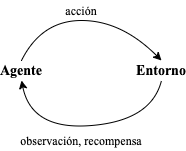
\includegraphics[width=0.3\textwidth]{cap2_contextualizacion/images/gym_ML.png}
    \caption{Interacción entorno-agente.}
    \label{fig:gym_ML}
\end{figure}

 El agente puede: 
 \begin{enumerate}
     \item \textbf{Conocer el modelo}: se conocen completamente todas las características del entorno. El aprendizaje en estos casos es mucho más sencillo, y la función óptima en estos problemas se alcanzan mediante la \textit{programación dinámica}. 
     \item \textbf{No conocer el modelo}: el entorno es desconocido, por lo que el aprendizaje es más costoso y además de adaptar la función óptima, se debe estudiar el modelo explícitamente en el algoritmo. Esta situación es la tratada en el trabajo realizado. 
 \end{enumerate}

Para poder elegir la acción óptima para cada estado determinado, el agente dispone de una política interna $\pi(s)$, unas guías que tienen como objetivo maximizar el total de recompensas en el tiempo. Cada estado está asociado a una función de valor $V(s)$ que predice el total esperado de recompensas futuras en este estado si actuamos de acuerdo con la política. \\


La interacción entre el agente y el entorno engloba una secuencia de acciones y recompensas observadas en el tiempo, $t = 1, 2,... T$. Durante el proceso, el agente acumula conocimientos sobre el entorno, aprende la política óptima y realiza decisiones sobre qué acción realizar a continuación para aprender eficientemente la mejor política. La secuencia de interacciones se identifica como \textbf{episodio}. El episodio siempre acabará en un estado final $S_T$. 


\subsubsection{Los elementos del aprendizaje por refuerzo}

En el siguiente apartado se utilizará $\mathbb{P}$ como la función de probabilidad y $\mathbb{E}$ como la suma de elementos. \\

 El modelo sirve para describir el entorno, y mediante éste se puede llegar a conocer la manera en la que el entorno interactúa y proporciona recompensas al agente. Las dos partes más importantes del modelo son la función de probabilidad $\mathbb{P}$ y la función de recompensa $R$.\\ 
 
 Estando en un estado $s$ se decide tomar una acción $a$ para llegar al siguiente estado $s'$ y obtener una recompensa $r$. Esto se conoce como una \textbf{transición}, y se representa por la tupla $(s, a, s', r)$. La función de transición guarda la probabilidad de transición de un estado $s$ a $s'$ tras la realización de $a$ y obteniendo una recompensa $r$.

\[ P(s', r|s, a) = \mathbb{P}[S_{t+1} = s', R_{t+1} = r |S_t = s, A_t = a] \]


La función de transición de estado se puede definir como una función de $P(s', r|s, a)$:
\[ P^a_{ss'} = P(s'|s, a) =\mathbb{P}[S_{t+1} = s'|S_t = s, A_t = a] = \sum_{r \in R} P(s', r|s, a) \]

La función de recompensa predice la siguiente recompensa tras la realización de una acción: 
\[ R(s,a) = \mathbb{E}[R_{t+1}|S_t = s, A_t=a]=\sum_{r \in R} r \sum_{s' \in S}P(s', r|s, a) \]

\subsubsection{La política}

La política $\pi$ define el comportamiento del agente; por lo tanto, es la responsable de determinar la acción a tomar en el estado $s$. La política se puede interpretar como un \textit{mapeo} del estado $s$ a la acción $a$ y puede ser:
\begin{itemize}
    \item \textbf{Determinista}: $\pi(s)=a$
    \item \textbf{Estocástica}: $\pi(a|s)=\mathbb{P}_\pi[A=a|S=s]$
\end{itemize}

\subsubsection{La función de valor}
Dicha función sirve para predecir la recompensa de un estado en concreto dada una acción. La recompensa predicha es la suma de las todas las \textit{recompensas descontadas} que se pueden obtener estando en un estado concreto. Esta acumulación se conoce como \textbf{retorno} $G_t$: 

\[ G_t = R_{t+1} + \gamma R_{t+2} + \ldots = \sum_{k = 0}^{\infty} \gamma^k R_{t+k+1} \]

El factor de descuento $\gamma \in$ [0, 1] sirve para penalizar las recompensas futuras. Tal como se explica en \cite{lilLogRL}, el motivo por el que se aplica este factor es debido a que: 
\begin{enumerate}
    \item Las recompensas futuras pueden ser inciertas.
    \item Las recompensas futuras no proporcionan beneficio inmediato. 
\end{enumerate}

El \textbf{estado-valor} del estado $s$ es el retorno esperado estando en el estado en un momento en el tiempo $t$, $S_t = s$:
\[V_\pi(s) = \mathbb{E}_\pi[G_t|S_t=s]\]

El \textbf{acción-valor} (también conocido como valor Q, o \textbf{Q-value} en inglés) se define como:
\[Q_\pi(s, a)=\mathbb{E}_\pi[G_t|S_t = s, A_t=a]\]

\subsubsection{La política y la función de valor óptimas}

La función de valor óptima produce el máximo retorno:
\[V_*(s)= \max_{\pi}V_\pi(s), Q_*(s, a)=\max_\pi Q_\pi(s, a)\]

La política óptima que proporciona las funciones de valor óptimas:
\[\pi_*=\arg\max_\pi V_\pi(s), \pi_* = \arg\max_\pi Q_\pi(s, a)\]

\subsubsection{Procesos de decisión de Markov}

Los problemas de aprendizaje por refuerzo son un tipo de \textbf{proceso de decisión de Markov} (MDP) \ref{fig:mdp}, ya que las recompensas futuras sólo dependen del estado actual. Por lo tanto, el pasado y el futuro son \textit{independientes} dados el presente - el estado actual del entorno proporciona suficiente información para decidir el futuro. \\

\begin{figure}[h]
    \centering
    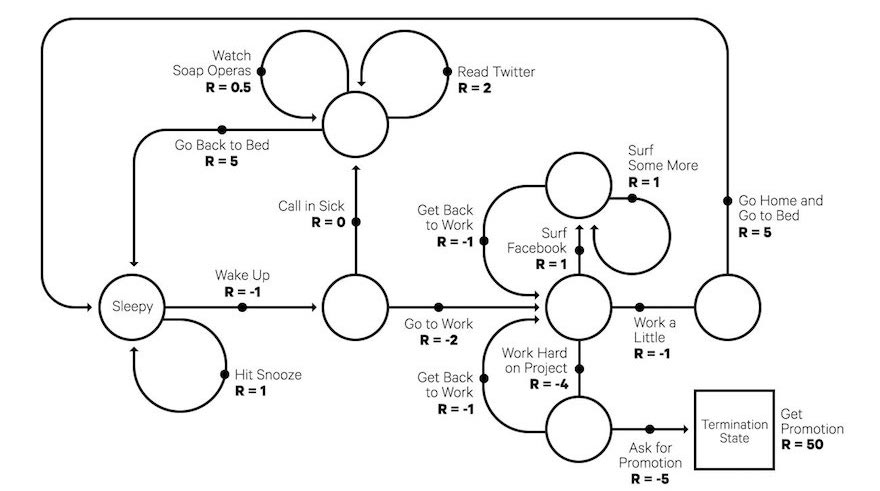
\includegraphics[width=0.9\textwidth]{cap2_contextualizacion/images/mdp.jpg}
    \caption{Ejemplo de un proceso de decisión de Markov. Fuente: \cite{randomantRL}}
    \label{fig:mdp}
\end{figure}

El proceso de decisión de Markov se compone por 5 elementos $M = \langle S, A, P, R, \gamma \rangle$, y se adaptan perfectamente a los conceptos previamente explicados:

\begin{itemize}
    \item $S$: Conjunto de estados.
    \item $A$: Conjunto de acciones.
    \item $P$: Función de probabilidad de transición.
    \item $R$: Función de recompensa.
    \item $\gamma$: Factor de descuento para recompensas futuras.
\end{itemize}

\subsubsection{Las ecuaciones Bellman}

Son un conjunto de ecuaciones que dividen la función de valor en las recompensas inmediatas y los valores futuros descontados. 

\begin{equation*}
\begin{split}
    V(s) & = \mathbb{E}[G_t|S_t = s]\\
    & = \mathbb{E}[R_{t+1} + \gamma R_{t+2} + \gamma^2 R_{t+3} + \ldots|S_t = s] \\
    & = \mathbb{E}[R_{t+1} + \gamma(R_{t+2} + \gamma R_{t+3} + \ldots)|S_t = s]\\
    & = \mathbb{E}[R_{t+1} + \gamma G_{t+1}|S_t = s]\\
    & = \mathbb{E}[R_{t+1} + \gamma V(S_{t+1})|S_t = s]
\end{split}
\end{equation*}

Y para el Q-value, 

\begin{equation*}
\begin{split}
   Q(s, a) & = \mathbb{E}[R_{t+1} + \gamma V(S_{t+1})|S_t = s, A_t = a] \\
   & = \mathbb{E}[R_{t+1} + \gamma \mathbb{E}_{a\sim \pi}Q(S_{t+1}, a)|S_t = s, A_t = a]
\end{split}
\end{equation*}

\paragraph{Ecuaciones Bellman de expectativa}
El proceso recursivo de actualización de la política se puede descomponer en ecuaciones de estado-valor y acción-valor. Con cada acción realizada en el entorno, se van propagando e $V$ y $Q$ mediante la misma política $\pi$.

\begin{figure}[h]
    \centering
    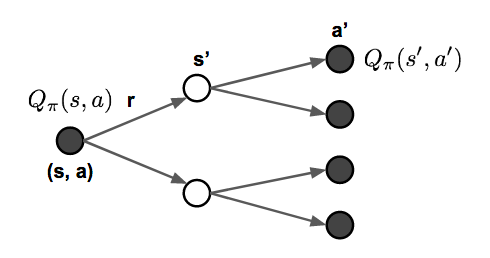
\includegraphics[width=0.6\textwidth]{cap2_contextualizacion/images/bellman_equation_expectation.png}
    \caption{Ilustración de cómo se actualizan las funciones estado-valor y acción-valor con las ecuaciones Bellman de expectativa. Fuente: \cite{lilLogRL}}
    \label{fig:bellman_equation_expectation}
\end{figure}

\[V_\pi(s)=\sum_{a \in A} \pi(a|s)Q_\pi(s,a)\]
\[Q_\pi(s,a) = R(s, a) + \gamma \sum_{s' \in S} P_{ss'}^a V_\pi(s')\]
\[V_\pi(s)=\sum_{a \in A} \pi(a|s)(R(s, a) + \gamma \sum_{s' \in S} P_{ss'}^a V_\pi(s'))\]
\[Q_\pi(s,a) = R(s, a) + \gamma \sum_{s' \in S} P_{ss'}^a \sum_{a' \in A} \pi(a'|s')Q_\pi(s',a')\]

\paragraph{Ecuaciones Bellman de optimalidad}

Si no se desean calcular los valores esperados mediante la política del agente, se calculan directamente los retornos máximos (y, por lo tanto, óptimos) obtenidos por las actualizaciones que no emplean la política. 

\[V_*(s)=\max_{a \in A}Q_*(s,a)\]
\[Q_*(s,a) = R(s, a) + \gamma \sum_{s' \in S} P_{ss'}^a V_*(s')\]
\[V_*(s)=\max_{a \in A}(R(s, a) + \gamma \sum_{s' \in S} P_{ss'}^a V_*(s'))\]
\[Q_*(s,a) = R(s, a) + \gamma \sum_{s' \in S} P_{ss'}^a \max_{a' \in A}Q_*(s',a')\]

No siempre es posible aplicar las ecuaciones Bellman ya que muchas veces no se conocen $P_{ss'}^a$ o $R(s,a)$. Sin embargo, estas ecuaciones plantean las bases teóricas de muchos algoritmos de aprendizaje por refuerzo \cite{lilLogRL}.

\subsubsection{Algoritmos de aprendizaje}

A continuación se explican los enfoques y algoritmos más usuales en el aprendizaje por refuerzo.  

\paragraph{Programación dinámica} Empleado cuando el modelo se conoce.  Se aplican las ecuaciones Bellman directamente para iterativamente evaluar las funciones de valor y mejorar la política del agente. 

La evaluación de la política $\pi$ se realiza mediante la ecuación de estado-valor $V_\pi$:
\[V_{t+1}(s)=\mathbb{E}_\pi[r + \gamma V_t(s')|S_t=s]=\sum_a \pi(a|s)\sum_{s', r}P(s', r|s, a)(r + \gamma V_t(s'))\]

A partir de la evaluación anterior se actualiza la política $\pi' \geq \pi$ de manera \textit{greedy} para generar una más eficiente.

\[Q_\pi(s, a) = \mathbb{E}[R_{t+1} + \gamma V_\pi(S_{t+1})|S_t = s, A_t = a] = \sum_{s', r}P(s', r|s, a)(r + \gamma V_\pi(s'))\]

La iteración de este proceso de evaluación y actualización de la política se emplea para mejorar la política. Dicha técnica se denomina \textbf{Iteración de Política Generalizada} (las siglas en inglés GPI). 

\[\pi_0 \overset{evaluar}{\longrightarrow} V_{\pi_0} \overset{actualizar}{\longrightarrow} \pi_1 \overset{evaluar}{\longrightarrow} V_{\pi_1} \overset{actualizar}{\longrightarrow} \pi_2 \overset{evaluar}{\longrightarrow} \ldots  \overset{actualizar}{\longrightarrow} \pi_* \overset{evaluar}{\longrightarrow} V_*\]

La función de valor se aproxima cada vez al valor real de la política mientras que la política se mejora constantemente para alcanzar la optimalidad. Supongamos que tenemos una política $\pi$ y la actualizamos de manera \textit{greedy} para obtener una política mejorada $\pi'$, $\pi'(s)=\arg \max_{a\in A}Q_\pi(s, a)$. El valor de $\pi'$ necesariamente será mejor porque:

\begin{equation*}
\begin{split}
   Q_\pi(s, \pi'(s)) & = Q_\pi(s, \arg \max_{a \in A} Q_\pi(s, a)) \\
   & = \max_{a \in A}Q_\pi(s, a) \geq Q_\pi (s, \pi(s)) = V_\pi(s)
\end{split}
\end{equation*}

\paragraph{Algoritmos de Monte Carlo} El aprendizaje mediante estos algoritmos se realiza a partir de los episodios de experiencia \textbf{completos} sin modelar las características del entorno, y se calcula el retorno medio observado como una \textit{aproximación} del retorno esperado. \\

Se debe tener en cuenta que $V(s = \mathbb{E}[G_t|S_t = s])$, $G_T = \sum_{k=0}^{T-t-1} \gamma^k R_{t+k+1}$, y que un episodio es ($S_1, A_1, R_2 \ldots, S_T$) y todos los episodios deben acabar.

El retorno empírico para un estado $s$ es:
\[V(s) = \frac{\sum_{t=1}^{T} \mathbb{1}[S_t = s]G_t}{\sum_{t=1}^{T} \mathbb{1}[S_t = s]}\]

donde $\mathbb{1}[S_t = s]$ es una función para indicar resultados en términos binarios. La aproximación se puede realizar mediante funciones de acción-valor mediante el recuento de parejas (s, a).

\[Q(s, a) = \frac{\sum_{t=1}^{T} \mathbb{1}[S_t = s, A_t = a]G_t}{\sum_{t=1}^{T} \mathbb{1}[S_t = s, A_t=a]}\]

Para aprender la política óptima mediante algoritmos de MC, se realiza una interación similar a la empleada en GPI.

\begin{enumerate}
    \item Actualizar la política de manera \textit{greedy} $\pi(s) = \arg \max_{a \in A} Q(s, a)$.
    \item Generar un nuevo episodio con la nueva política $pi$.
    \item Estimar Q utilizando el nuevo episodio: $q_\pi(s, a)= \frac{\sum_{t=1}^{T} (\mathbb{1}[S_t=s, A_t=a] \sum_{k=0}^{T-t-1} \gamma^{k} R_{t+k+1})}{\sum_{t=1}^{T} \mathbb{1}[S_t=s, A_t = a]}$
\end{enumerate}

\paragraph{Algoritmos de diferencia temporal} En inglés \textit{Temporal Difference} (TD), es parecido a los métodos de MC ya que no estudian el modelo y aprenden de los episodios de la experiencia. Sin embargo, en TD el aprendizaje se realiza con episodios \textbf{incompletos}, por lo que no es necesario monitorizar los episodios hasta que se terminen. \\

Los métodos TD actualizan unos \textit{targets} empleando estimaciones existentes en vez de centrarse exclusivamente en recompensas actuales y retornos completos como en MC. Este métodos se conocen como \textbf{bootstrapping}. \\

La idea principal en TD es actualizar $V(S_t)$ para aproximarse al retorno $R_{t+1} + \gamma V(S_{t+1})$ (conocido como target TD). El nivel de actualización de la función de valor se controla mediante un parámetro de aprendizaje (en inglés \textit{learning rate}) $\alpha$:

\begin{equation*}
\begin{split}
   V(S_t) &\leftarrow (1 - \alpha)V(S_t) + \alpha G_t \\
   V(S_t) &\leftarrow V(S_t) + \alpha(G_t - V(S_t)) \\
   V(S_t) &\leftarrow V(S_t) + \alpha(R_{t+1} + \gamma V(S_{t+1}) - V(S_t))
\end{split}
\end{equation*}

Para la función de acción-valor: 

\[Q(S_t, A_t) \leftarrow Q(S_t, A_t) + \alpha(R_{t+1} + \gamma Q(S_{t+1}, A_{t+1})) - Q(S_t, A_t))\]

En cuanto a la optimización de la política, existen distintos métodos que se emplean en los algoritmos TD de acuerdo con \cite{lilLogRL}:

\begin{itemize}
    \item \textbf{SARSA}: parecido a GPI. Se actualiza el Q-value siguiendo una secuencia de $\ldots, S_t, A_t, R_{t+1}, S_{t+1}, A_{t+1}, \ldots$. En un episodio:
    \begin{enumerate}
        \item Inicializar $t=0$.
        \item Empezar con $S_0$ y elegir la acción $A_0 = \arg \max_{a \in A} Q(S_0, a)$.
        \item En el instante de tiempo $t$, tras aplicar la acción $A_t$, observar la recompensa $R_{t+1}$ y hacer la transición al siguiente estado $S_{t+1}$.
        \item Elegir la siguiente acción como en el paso 2: $A_{t+1} = \arg \max_{a \in A} Q(S_{t+1}, a).$
        \item Actualizar la función Q-value:
        \[Q(S_t, A_t) \leftarrow Q(S_t, A_t) + \alpha(R_{t+1} + \gamma Q(S_{t+1}, A_{t+1}) - Q(S_t, A_t))\]
        \item Incrementar el tiempo $t = t + 1$ y repetir el proceso a partir del paso 3. 
    \end{enumerate}
    En cada iteración del SARSA, se debe elegir la \textit{siguiente} acción teniendo en cuenta la política \textit{actual}. 
    \item \textbf{Q-Learning}: a diferencia de SARSA no sigue la política actual para elegir la siguiente acción. Hace una estimación de $Q^*$ eligiendo los mejores valores Q, pero la acción $a^*$ que lleva a este valor máximo de Q no es importante y en el siguiente paso de Q-learning puede que no se escoja $a*$ como la acción a tomar.
    \begin{enumerate}
        \item Inicializar $t=0$.
        \item Empezar con $S_0$.
        \item En el instante de tiempo $t$ se elige una acción teniendo en cuenta los Q-values, $A_t = \arg \max_{a \in A} Q(S_t, a)$ y $\epsilon$-greedy se suele aplicar. 
        \item Tras aplicar la acción $A_t$, observar la recompensa $R_{t+1}$ y hacer la transición al siguiente estado $S_{t+1}$. 
        \item Elegir la siguiente acción como en el paso 2: $A_{t+1} = \arg \max_{a \in A} Q(S_{t+1}, a).$
        \item Actualizar la función Q-value: 
        \[Q(S_t, A_t) \leftarrow Q(S_t, A_t) + \alpha(R_{t+1} + \gamma \max_{a \in A}Q(S_{t+1},a) - Q(S_t, A_t))\]
        \item $t = t + 1$ y repetir el proceso a partir del paso 3. 
    \end{enumerate} 
    \begin{figure}[h]
    \centering
    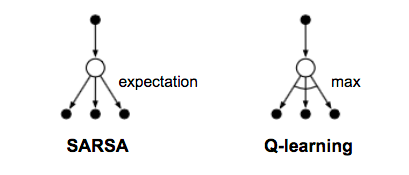
\includegraphics[width=0.5\textwidth]{cap2_contextualizacion/images/sarsa_vs_q_learning.png}
    \caption{Diagramas SARS y Q-Learning. Fuente: \cite{lilLogRL}}
    \label{fig:sarsa_vs_q_learning}
    \end{figure}
    Para poder evitar problemas de memoria y evitar tener guardadas todas las parejas de estado-acción, se emplean funciones de aproximación para determinar los Q-values. La función se identifica con $Q(s, a; \theta)$. \\
    
    Sin embargo, este algoritmo puede ser inestable y no llegar a converger si se utiliza una función de Q-value no linear y el método de \textit{bootstrapping}. 
    \begin{figure}[h]
    \centering
    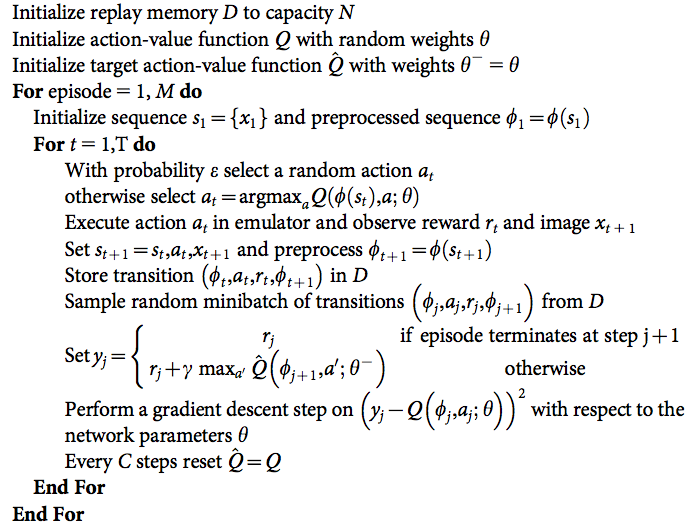
\includegraphics[width=0.7\textwidth]{cap2_contextualizacion/images/DQN_algorithm.png}
    \caption{Algoritmo DQN con repetición de experiencia y actualización de target. (Fuente: \cite{lilLogRL})}
    \label{fig:DQN_algorithm}
    \end{figure}
    \item \textbf{Deep Q-Learning}\label{dqn-learning}: mejora del \textit{Q-Learning} que introduce dos mecanismos nuevos para estabilizar el proceso de entrenamiento: la \textbf{repetición de experiencia} (\textit{experience replay}) y la \textbf{actualización periódica del target}. 
    \begin{itemize}
        \item \textit{Repetición de experiencia:} \label{dqn-learning-replay} todos los episodios $e_t = (S_t, A_t, R_t, S_(t+1))$ se guardan en la memoria de repetición $D_t = {e_1, \ldots, e_t}$. $D_t$ contiene las tuplas de la experiencia de distintos episodios. Durante la actualización de los Q-values, se toman muestras aleatorias de la memoria de repetición. Este método mejora la eficiencia de datos ya que se utiliza la misma experiencia más de una vez, elimina las correlaciones entre las secuencias de observaciones, y suaviza los cambios en la distribución de datos. 
        \item \textit{Actualización periódica del target}: Q se optimiza para acercarse a unos valores concretos que se actualizan periódicamente. La red se clona y se mantiene como el target de optimización cada $C$ iteraciones. Esta modificación hace que el entreno sea más estable ya que elimina las oscilaciones a corto plazo. \\
        
        La función de error es: 
        
        \[L(\theta) = \mathbb{E}_{(s, a, r, s') \sim U(D)}[(r + \gamma \max_{a'} Q(s', a'; \theta^-) - Q(s, a; \theta))^2]\]
         donde $U(D)$ es la distribución uniforme de la memoria de repetición $D$; $\theta^-$ son los parámetros mantenidos de la red Q empleada como target.  
    \end{itemize}

\end{itemize}

\subsubsection{Exploración y explotación} \label{explorationExploitation}

Al encontrar un entorno desconocido, es evidente la necesidad de explorarlo sin seguir ningún criterio ya que no se dispone de conocimientos sobre cómo actuar. Una vez nos familiaricemos con el entorno, ya no hace falta explorar tanto sino que deberíamos aprovechar los conocimientos adquiridos ya que en principio, además de ser correctos, nos llevan a buenas recompensas. \\

Lo descrito anteriormente es la \textbf{exploración} y la \textbf{explotación}, y el agente debe combinar ambas para poder asegurar que consigue una solución óptima. Si no \textit{explora} suficientemente no tendrá conocimientos para saber actuar dentro del entorno, pero si en cambio no \textit{explota} los conocimientos tras adquirirlos puede estar arriesgándose a explorar otras opciones que pueden que no lleven al objetivo. 


\section{El enfoque ascendente y las redes neuronales}

El enfoque ascendente, también conocido como \textit{conexionismo} o \textit{computación neuronal}, se ha desarrollado como un intento de entender cómo funciona el cerebro humano a nivel neuronal y, más concretamente, cómo las personas \textit{aprenden} y son capaces de \textit{recordar}. \\

En 1943, el neurólogo Warren McCulloch y el matemático Walter Pitts publicaron un trabajo \cite{mcculloch1943logical} sobre las redes neuronales en el cual se exponía que una neurona del cerebro \textbf{es como un procesor digital}, y que el cúmulo de éstas componen \textbf{una máquina computacional}; al fin y al cabo, el cerebro es un sistema que \textit{calcula} acciones que el humano debe tomar. Discutiendo sobre sus investigaciones, McCulloch señaló

\begin{displayquote}\textit{
What we thought we were doing (and I think we succeeded fairly well) was treating the brain as a Turing machine.}
\end{displayquote}

\subsection{Creación de una red neuronal}

La primera red neuronal fue creada años después, en 1954 (Belmont Farley y Wesley Clark). Contaba con un \textbf{total de 128 neuronas y era capaz de reconocer patrones sencillos}. Además, se descubrió que aunque se eliminen menos del 10\% del total de neuronas de la red entrenada, su eficacia y rendimiento no se verían afectados; este hecho recuerda a cómo el cerebro puede sufir daños leves tras sufrir una operación, un accidente o una enfermedad y mantener sus capacidades. \\

\begin{figure}[h]
    \centering
    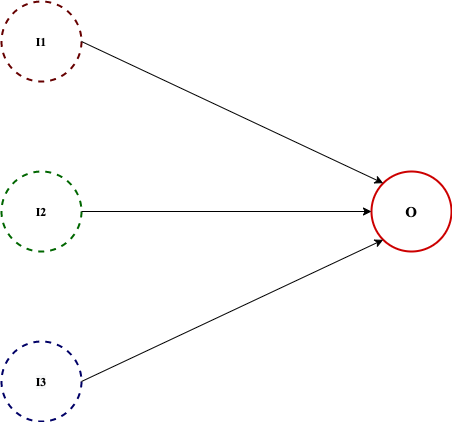
\includegraphics[scale=0.35]{cap2_contextualizacion/images/red_neuronal.png}
    \caption{Red neuronal simple.}
    \label{fig:red_neuronal_simple}
\end{figure}

En la Fig. ~\ref{fig:red_neuronal_simple} se muestra una simple red neuronal que consta de 4 neuronas - las neuronas \textbf{\textit{I1}}, \textbf{\textit{I2}} e \textbf{\textit{I3}} corresponden a las neuronas de entrada (\textit{input}) y todas se conectan a la neurona \textbf{\textit{O}}, la neurona de salida (\textit{output}). \\

El funcionamiento de una red neuronal es sencillo - la información se va transfiriendo por las neuronas por medio de \textit{estímulos} que van activando o desactivando las neuronas que componen la red. Para que una neurona \textbf{se active} (también se hace el símil de que la neurona se \textit{dispara}), debe recibir unos estímulos de las neuronas a las que ya están conectadas. La neurona interpreta este estimulo de dos maneras: o bien activándose y transfiriendo dicha estimulación a las neuronas conectadas o, de lo contrario, permaneciendo desactivada y acabando dicha interacción. 

Un estímulo de una neurona se calcula \textbf{teniendo en cuenta todas las neuronas} activas que están conectadas a la neurona de salida, es decir, la que se desea activar a continuación. Cada conexión entre las neuronas de entrada y salida tiene un peso $\omega$, y la suma ponderada de los pesos es el estímulo total. Para que una neurona se active este estímulo debe ser mayor o igual al umbral de activación $\theta$ de la neurona. \\

A continuación se describirá un ejemplo de este funcionamiento considerando que:

\begin{enumerate}
    \item La neurona O tendrá un umbral de activación de \textbf{4}.
    \item La conexión entre la neurona \textit{I1} y la \textit{O} tiene un peso de \textbf{1}.
    \item El peso entre la \textit{I2} y \textit{O} es \textbf{2.75}.
    \item El peso entre \textit{I3} y \textit{O} es \textbf{0.25}.
\end{enumerate} 

En la Fig. ~\ref{fig:red_neuronal_activacion} se plantean 2 casos distintos: 

\begin{enumerate}
    \item En la Fig. ~\ref{fig:red_neuronal_inactiva}, las neuronas \textit{I1} e \textit{I2} están activas pero la \textit{I3} está inactiva. La suma ponderada de los pesos está por debajo del umbral de activación de la neurona \textit{O}, por lo que no se activará. 
    \item En la Fig. ~\ref{fig:red_neuronal_activa}, todas las neuronas están activas y la suma ponderada de los pesos es igual al umbral de activación de \textit{O}, por lo que ésta se activará.
\end{enumerate}

\begin{figure}[h]
    \centering
    \begin{subfigure}{.45\textwidth}
        \centering
        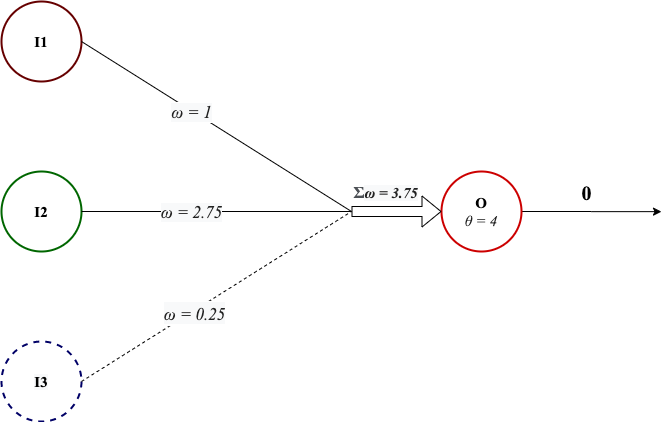
\includegraphics[scale=0.22]{cap2_contextualizacion/images/red_neuronal_inactive.png}
        \caption{I3 inactivo, suma ponderada por debajo del umbral de activación de O.}
        \label{fig:red_neuronal_inactiva}
    \end{subfigure}      
    \begin{subfigure}{.45\textwidth}
        \centering
        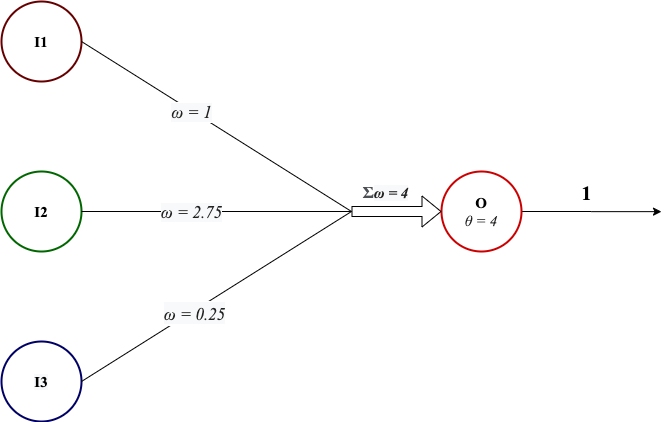
\includegraphics[scale=0.22]{cap2_contextualizacion/images/red_neuronal_active.png}
        \caption{I1, I2, I3 activas, suma ponderada igual al umbral de activación de O.}
        \label{fig:red_neuronal_activa}
    \end{subfigure}
    \caption{Activación de la neurona O según las neuronas activas de entrada.}
    \label{fig:red_neuronal_activacion}
\end{figure}

\subsection{Entreno de una red neuronal}

Las redes neuronales son ampliamente usadas en las tareas de predicción y de clasificación. Sin embargo, como paso previo a estas tareas es necesario \textit{\textbf{entrenar}} la red. El proceso de entreno sirve para que la red \textit{adquiera experiencia} con los datos, de modo que será capaz de reconocer, clasificar y/o predecir el resultado adecuado con cada dato que se le presenta. \\

En el entreno es necesario disponer de un \textit{conjunto de datos de entrenamiento}. Este \textit{dataset} estará compuesto por distintas muestras - parejas de datos de entrada y de salida con las que la red aprenderá cuáles son las interpretaciones correctas. \\

En cuanto al proceso, el entreno consiste en los siguientes pasos: 
\begin{enumerate}
    \item El agente externo presenta un ejemplo de patrón a la red y observa el comportamiento de \textit{O}.
    \item El agente ajusta los pesos de las conexiones en función de estas dos normas:
        \begin{enumerate}
        \item Si el resultado es 0 pero se deseaba una salida de 1, se \textbf{incrementa} el peso de todas las conexiones de las neuronas \textit{activas} que conducen a O (y así se incrementa las probabilidades de que O se active cuando se presenten las mismas condiciones).
        \item Si el resultado es 1 pero se deseaba una salida de 0, se \textbf{decrementa} el peso de todas las conexiones de las neuronas \textit{activas} que conducen a O (y así se incrementa las probabilidades de que O se active cuando se presenten las mismas condiciones).
    \end{enumerate}
\end{enumerate}

Este proceso se realiza varias iteraciones, en cada iteración aplicando este proceso de dos paso a cada muestra del \textit{dataset}. De esta manera se obtiene un \textit{patrón de pesos} sobre las conexiones que posibilita a la red ofrecer una respuesta a todos los ejemplos ofrecidos. \\